%Section3.tex

%%%%%%%%%%%%%%%%%%%%%%%%%%%%%%%%%%%%%%%%%%%%%%%%%%%%%%%%%%%%%%%%%%%%%%%%%%%%%%%%%
\section{Real root location}\label{S:three}
%
%
The remaining methods in  \texttt{RealRoots} are linear-algebraic any may be used to cont real zeroes of an ideal $I$ in
$\RR^n$ according to the sign of another polynomial, similar to Sylvester's Theorem~\ref{Th:Sylvester}.
We demonstrate how this may be used for real root location and comment on its applicability over other fields.
 this for the ideal $I$ of Section~\ref{S:two}.
Let
\[
f\ vcentcolon=\ 5-3x^2-3y^2+x^2y^2\,,
\ \quad
g\ \vcentcolon=\ 1+2xy-4xy^2+3x^2y\,.
\]


(This is for my real root location example and discussion)
\[
\fbox{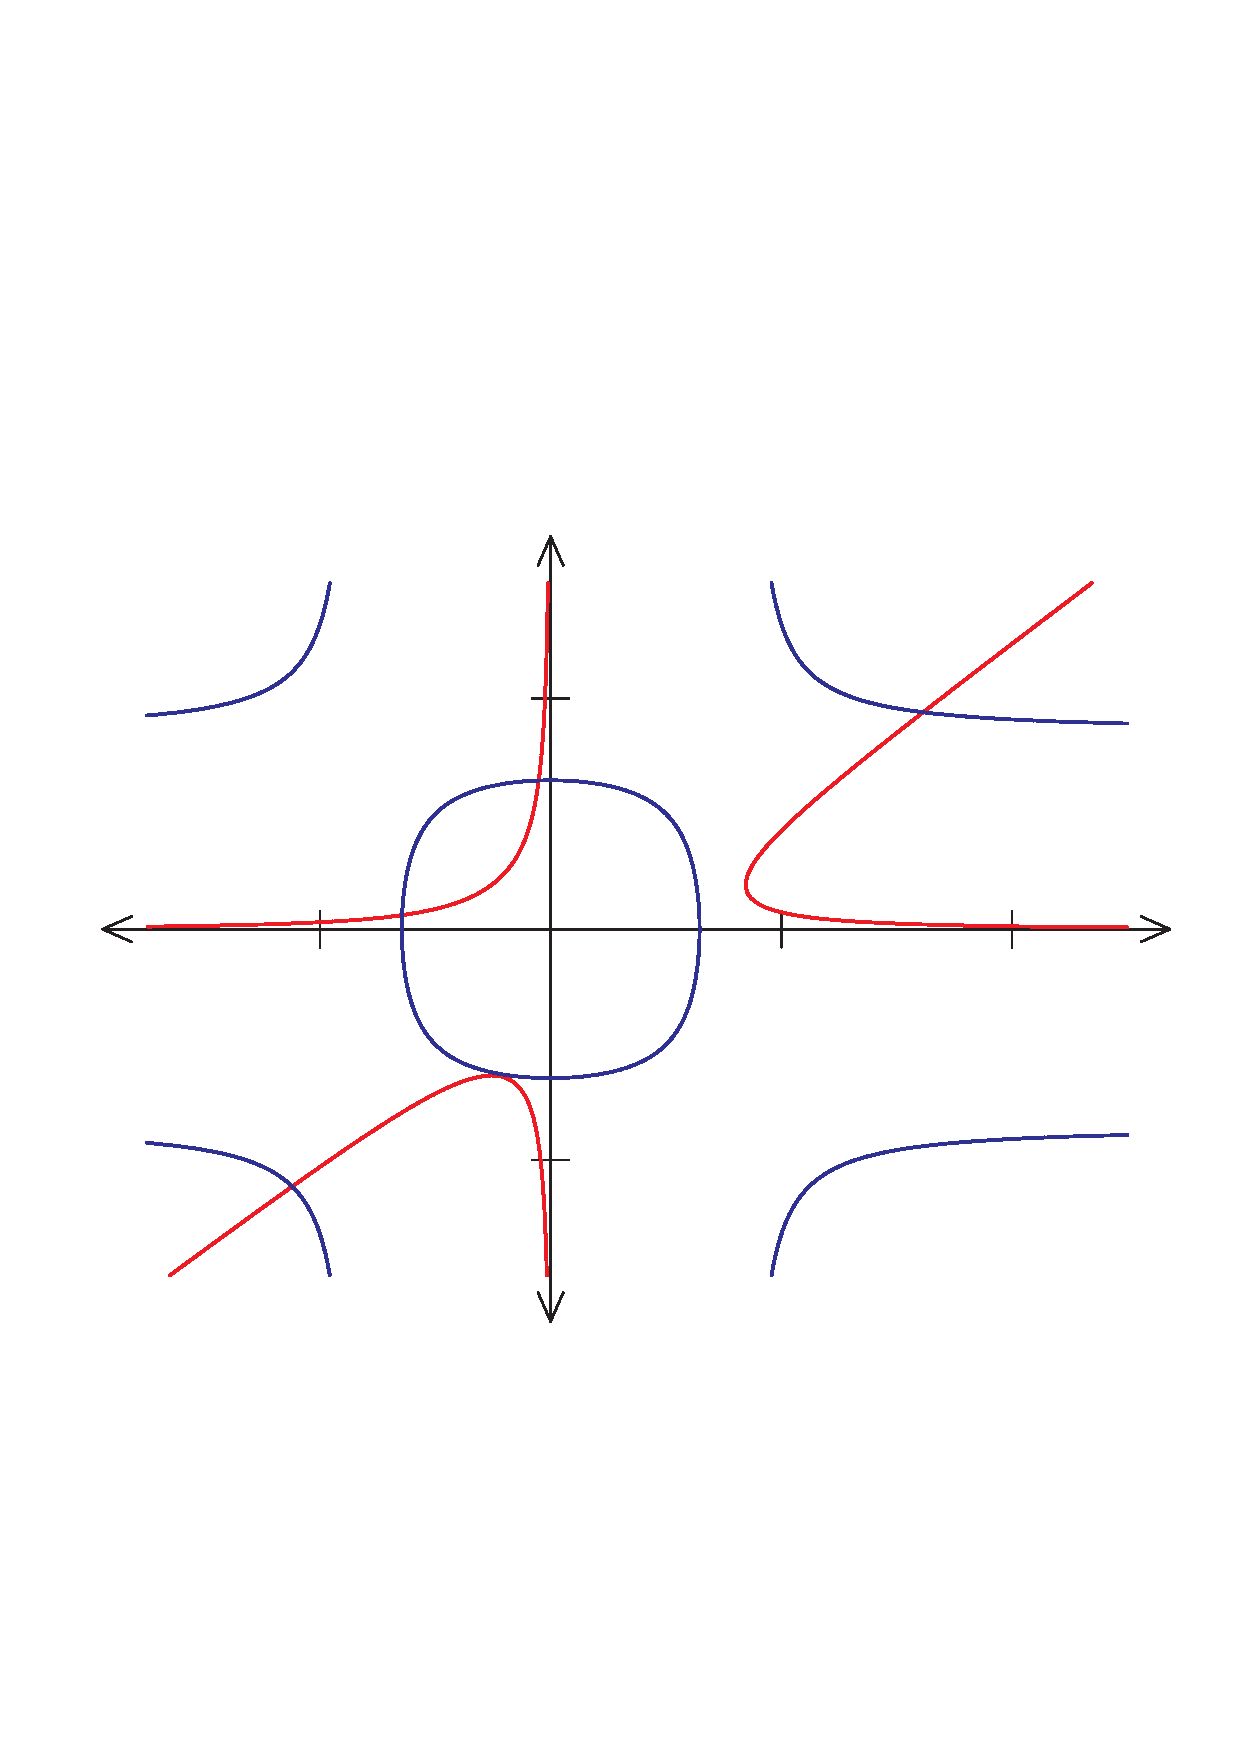
\includegraphics[height=120pt]{pictures/TwoCurves}}
\]
%Trace form is Thm 4.72 in BPR
%
%Sylvester's theorem  is Thm. 2.55 in BPR
%
\newpage
